% !TEX TS-program = pdflatex
% !TEX encoding = UTF-8 Unicode

% This is a simple template for a LaTeX document using the "article" class.
% See "book", "report", "letter" for other types of document.

\documentclass[11pt]{article} % use larger type; default would be 10pt

\usepackage[utf8]{inputenc} % set input encoding (not needed with XeLaTeX)

%%% Examples of Article customizations
% These packages are optional, depending whether you want the features they provide.
% See the LaTeX Companion or other references for full information.

%%% PAGE DIMENSIONS
\usepackage{geometry} % to change the page dimensions
\geometry{a4paper} % or letterpaper (US) or a5paper or....
% \geometry{margin=2in} % for example, change the margins to 2 inches all round
% \geometry{landscape} % set up the page for landscape
%   read geometry.pdf for detailed page layout information

\usepackage{graphicx} % support the \includegraphics command and options

% \usepackage[parfill]{parskip} % Activate to begin paragraphs with an empty line rather than an indent

%%% PACKAGES
\usepackage{booktabs} % for much better looking tables
\usepackage{array} % for better arrays (eg matrices) in maths
\usepackage{paralist} % very flexible & customisable lists (eg. enumerate/itemize, etc.)
\usepackage{verbatim} % adds environment for commenting out blocks of text & for better verbatim
\usepackage{subfig} % make it possible to include more than one captioned figure/table in a single float
% These packages are all incorporated in the memoir class to one degree or another...

\usepackage{scrextend}
\usepackage{blindtext}
\addtokomafont{labelinglabel}{\sffamily}
\usepackage{graphicx}
\usepackage{fancyvrb}
\newcommand{\verbatimfont}[1]{\renewcommand{\verbatim@font}{\ttfamily#1}}

%%% HEADERS & FOOTERS
\usepackage{fancyhdr} % This should be set AFTER setting up the page geometry
\pagestyle{fancy} % options: empty , plain , fancy
\renewcommand{\headrulewidth}{0pt} % customise the layout...
\lhead{}\chead{}\rhead{}
\lfoot{}\cfoot{\thepage}\rfoot{}

%%% SECTION TITLE APPEARANCE
\usepackage{sectsty}
\allsectionsfont{\sffamily\mdseries\upshape} % (See the fntguide.pdf for font help)
% (This matches ConTeXt defaults)

%%% ToC (table of contents) APPEARANCE
\usepackage[nottoc,notlof,notlot]{tocbibind} % Put the bibliography in the ToC
\usepackage[titles,subfigure]{tocloft} % Alter the style of the Table of Contents
\renewcommand{\cftsecfont}{\rmfamily\mdseries\upshape}
\renewcommand{\cftsecpagefont}{\rmfamily\mdseries\upshape} % No bold!

\usepackage{hyperref}

%%% END Article customizations

%%% The "real" document content comes below...

\title{Project P7: Design an A/B Test}
\author{Peter Eisenschmidt}
%\date{} % Activate to display a given date or no date (if empty),
         % otherwise the current date is printed 



\begin{document}
\maketitle

\section{Experiment Design}

\subsection{Metric Choice}

The following metrics have been selected as \textbf{Invariant Metrics}:
\begin{labeling}{Click-through-probability}
\item [Number of cookies] The number of unique cookies to visit the page should not be affected by the experiment, as someone visiting the course overview page has not seen the changes yet. 
\item [Number of clicks] The same applies to the number of clicks on the "Start Free Trial" button; there should not be any impact of the experiment on this metric
\item [Click-through-probability] As the CTR is defined as the number of unique cookies to click the "Start free trial" button divided by the number of unique cookies to view the course overview page (both of which are invariant metrics), the click-through-probability is also an invariant metric
\end{labeling}
\noindent These three metrics are not impacted by the experiment and hence one can expect similar distributions between control and experiment groups.
\medskip
\noindent The following metrics have been selected as \textbf{Evaluation Metrics}:
\begin{labeling}{Gross conversion}
\item [Gross conversion] Being defined as the number of user-ids to complete checkout and enroll in the free trial divided by the number of unique cookies to click the "Start free trial" button, one would expect a lower gross conversion for the experiment as for the control group. The goal of the tested change is to reduce the number of frustrated students, so you could expect that students that are likely to drop out with the current design are filtered out early and do not complete the checkout.
\item [Retention] Similarly, you would expect an increased retention as a result of the experiment, as the number of students that complete the checkout should reduce. At the same time, the number of students to make at least one payment should remain the same.
\item [Net conversion] Net conversion is the combination of the two previously mentioned metrics. It is expected that net conversion does not decrease for both control and experiment group, as the number of students to remain enrolled past the 14-day boundary should not decrease significantly due to the experiment.
\end{labeling}
\noindent For each of these metrics, a practical significance boundary $d_{min}$ is defined. This indicates the minimum difference that needs to be observed between control and experiment group in order to determine whether the change is meaningful or not. This is important for the decision to whether or not launch the change.

For the above given evaluations metrics, the practical significance boundaries are $d_{min} = .01$ (for gross conversion and retention) and $d_{min} = .0075$ (for net conversion). \medskip

The following metrics have not been select as either \textbf{Invariant Metrics} or \textbf{Evaluation Metrics}:
\begin{labeling}{[Number of User IDs}
\item [Number of User IDs] Firstly, the number of users to enroll in the free trial are expected to change with the experiment, hence it cannot be an invariant metric. Secondly, it is not selected as an evaluation metric as the absolute number of users to enroll may vary based on external conditions, e.g. seasonal variations. Therefore it is better to use User ID as a normalized parameter, as in Gross Conversion.
\end{labeling}

\subsection{Measuring Standard Deviation}

The analytical estimate of the standard deviation can be calculated as follows:
\begin{equation}
     \sigma = \sqrt{\frac{p(1-p)}{N}}
\end{equation}
\noindent where the probabilities are given in the baseline values:
\begin{itemize}
\item Probability of enrolling, given click (Gross Conversion): $p= .20625$
\item Probability of payment, given enroll (Retention): $p=.5300$
\item Probability of payment, given click (Net Conversion): $p=0.1093125$
\end{itemize}

\noindent Given that the sample size to visit the course overview page is 5000 cookies, the number of units of analysis for each metric can be calculated as follows. For gross conversion, it is given by:
\begin{equation}
     N = \frac{PageViews \times Cookies_{ClickFreeTrial}}{Cookies_{ViewPagePerDay}} = \frac{5000 \times 3200}{40000} = 400
\end{equation}
For retention it can be calculated as:
\begin{equation}
     N = \frac{PageViews \times Enrollments}{Cookies_{ViewPagePerDay}} = \frac{5000 \times 660}{40000} = 82.5
\end{equation}
For net conversion, it is the same as gross conversion:
\begin{equation}
     N = \frac{PageViews \times Cookies_{ClickFreeTrial}}{Cookies_{ViewPagePerDay}} = \frac{5000 \times 3200}{40000} = 400
\end{equation}
This results in the following standard deviations:
\begin{itemize}
\item Gross Conversion: $\sigma = .0202$
\item Retention: $\sigma = .0549$
\item Net Conversion: $\sigma =  .0156$
\end{itemize}

For both gross and net conversion, the unit of analysis and the unit of diversion are the same (cookies), whereas the unit of analysis for retention is User ID. Therefore, the analytic estimate of the standard deviation is likely to be comparable to the empirical standard deviation for gross and net conversion but not for retention. For the latter it might be interesting to do an empirical estimate.

\subsection{Sizing}
\subsubsection{Number of Samples vs. Power}

In order to determine the number of samples, this calculator \url{http://www.evanmiller.org/ab-testing/sample-size.html} is used. For all three metrics, $1-\beta$ is 80\% and $\alpha$ is 5\%, i.e. no Bonferroni correction is applied. 

The baseline conversion rate and the minimum detectable effect $d_{min}$ is listed below for each metric as well as resulting number of samples.

\begin{itemize}
\item Gross conversion:
	\begin{itemize}
		\item Baseline conversion: 20.625\%
		\item Minimum detectable effect: 1\%
		\item Samples = 25,835
	\end{itemize}
\item Retention:
	\begin{itemize}
		\item Baseline conversion: 53\%
		\item Minimum detectable effect: 1\%
		\item Samples = 39,115
	\end{itemize}
\item Net conversion:
	\begin{itemize}
		\item Baseline conversion: 10.93125\%
		\item Minimum detectable effect: .75\%
		\item Samples = 27,413
	\end{itemize}
\end{itemize}
The number of pageviews can then be calculated as follows for gross and net conversion:
\begin{equation}
	N_{PV} = 2 \times n_{Samples} \times \frac{Cookies_{ViewPagePerDay}}{Cookies_{ClickFreeTrial}}
\end{equation}
For retention it is given by
\begin{equation}
	N_{PV} = 2 \times n_{Samples} \times \frac{Cookies_{ViewPagePerDay}}{Enrollments}
\end{equation}
The resulting page views are:
\begin{labeling}{Gross Conversion}
\item[Gross Conversion] 645,875
\item[Retention]  4,741,212
\item[Net Conversion]  685,325
\end{labeling}
Therefore, a total number of 4,741,212 page views is required if all metrics are to be used.

\subsubsection{Duration vs. Exposure}

The change tested in this experiment is a low risk for the participants (no collection of sensitive data, no exposure to physical harm as the change consists of asking the student how much time per week they were willing to invest in the course). Therefore, it can be assumed to be safe to divert 100\% of the traffic to this experiment. With 40,000 page views per day, this results in the following durations:

\begin{itemize}
\item Duration (Gross conversion): 17 days
\item Duration (Retention):        119 days
\item Duration (Net conversion):   18 days
\end{itemize}
119 days is not feasible for this experiment, therefore retention is not retained as a metric. The resulting experiment duration is then 18 days.

\section{Experiment Analysis}
\subsection{Sanity Checks}

For \textbf{cookies}, there is a 50\% probability of being either in the control or in the experiment group. In the experiment and control group there were 344,660 and 345,543 page views respectively. The standard deviation is therefore:
\begin{equation}
	\sigma = \sqrt{\frac{2p}{N_{exp} + N_{cont}}} = .00060
\end{equation}
The margin of error (for a 95\% confidence interval, i.e. z = 1.96) is then:
\begin{equation}
	m = \sigma \times z = 0.00118
\end{equation}
Consquently, the upper and lower bound for cookies are 0.49882 and 0.50118 respectively.\medskip

The observed value is 
\begin{equation}
	p = \frac{N_{cont}}{N_{exp}+N_{cont}} = .50064
\end{equation}
which is in between the lower and upper bound.\medskip

For the \textbf{number of clicks}, the probability is also 50\%. The number of clicks in the experiment and the control group are 28325 and 28378 respectively. The resulting standard deviation is therefore:
\begin{equation}
	\sigma = \sqrt{\frac{2p}{N_{exp} + N_{cont}}} = .00210
\end{equation}
The margin of error is then:
\begin{equation}
	m = \sigma \times z = 0.00412
\end{equation}
Consquently, the upper and lower bound for number of clicks are .49588  and .50412 respectively.\medskip

The observed value is 
\begin{equation}
	p = \frac{N_{cont}}{N_{exp}+N_{cont}} = .50047
\end{equation}
which also falls within the boundaries of the confidence interval.\medskip

Lastly, the observed \textbf{Click-through-probability} of experiment and control group are .08219 and .08213 respectively. The standard deviation for the control group is
\begin{equation}
	\sigma = \sqrt{\frac{CTP_{cont}\times (1-CTP_{cont})}{N_{cont}}} = .00047
\end{equation}
and the margin of error:
\begin{equation}
	m = \sigma \times z = .00092
\end{equation}
which results in lower and upper bounds of .08121 and .08304. The CTP of the experiment group is within this confidence intervall.\medskip

It can therefore be concluded that all invariant metrics pass the sanity checks.

\subsection{Result Analysis}

\subsubsection{Effect Size Test}

The \textbf{Gross Conversion} of experiment and control group are:
\begin{eqnarray}
	GC_{exp} &=& \frac{X_{exp}}{N_{exp}} =  .19832\\
	GC_{cont} &=& \frac{X_{cont}}{N_{cont}}= .21887
\end{eqnarray}
where $X_{exp}$ and $X_{cont}$ are the number of enrollments in both groups. Please note that only rows are used where Enrollments are not null. This results in $N_{exp}=17,260$ and $N_{cont}=17,293$. \medskip

The observed difference is therefore:
\begin{equation}
	\hat{d} = GC_{exp} - GC_{cont} = -.02055
\end{equation}
The pooled probability is hence:
\begin{equation}
	\hat{p}_{pool} = \frac{X_{exp}+ X_{cont}}{N_{exp} + N_{cont}} = .20861
\end{equation}
The pooled standard error is then given by:
\begin{equation}
	SE_{pool} = \sqrt{\hat{p}_{pool}\times \left(1-\hat{p}_{pool}\right) \times \left(\frac{1}{N_{exp}} + \frac{1}{N_{cont}}\right)} = .00437
\end{equation}
which in turn gives a margin of error (with $z=1.96$ for a 95\% confidence interval):
\begin{equation}
	m = z \times SE_{pool} = .00857
\end{equation}
The confidence interval for \textbf{Gross Conversion} is therefore:
\begin{equation}
	CI = \left(-0.02912, -0.01199\right)
\end{equation}
This means that gross conversion is both statistically and practically significant (recall that the practical significance boundary is .01).\medskip

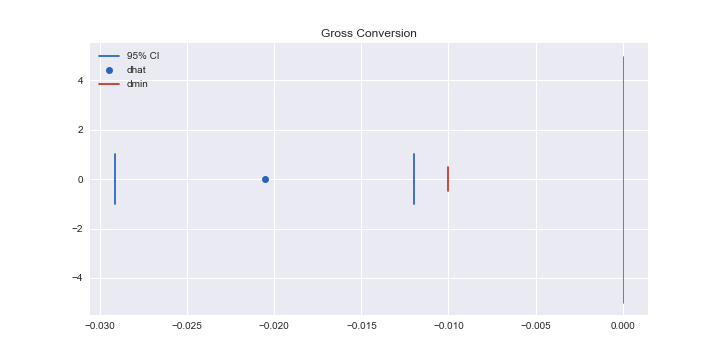
\includegraphics[width=\textwidth]{gross_conv}

Similarly, the \textbf{Net Conversion} of experiment and control group are:
\begin{eqnarray}
	NC_{exp} &=& \frac{X_{exp}}{N_{exp}} =  .11269\\
	NC_{cont} &=& \frac{X_{cont}}{N_{cont}}= .11756
\end{eqnarray}
where $X_{exp}$ and $X_{cont}$ are the number of payments in both groups. As before, only rows where payments are not null are used.

The observed difference is then:
\begin{equation}
	\hat{d} = NC_{exp} - NC_{cont} = -.00487
\end{equation}
The pooled probability is hence:
\begin{equation}
	\hat{p}_{pool} = \frac{X_{exp}+ X_{cont}}{N_{exp} + N_{cont}} = .11513
\end{equation}
The pooled standard error is then given by:
\begin{equation}
	SE_{pool} = \sqrt{\hat{p}_{pool}\times \left(1-\hat{p}_{pool}\right) \times \left(\frac{1}{N_{exp}} + \frac{1}{N_{cont}}\right)} = .00343
\end{equation}
which in turn gives a margin of error (with $z=1.96$ for a 95\% confidence interval):
\begin{equation}
	m = z \times SE_{pool} = .00673
\end{equation}
The confidence interval for \textbf{Net Conversion} is therefore:
\begin{equation}
	CI = \left(-0.01160, 0.00186\right)
\end{equation}
As zero is contained within the net conversion confidence intervall, the results are neither statistically or practically significant.

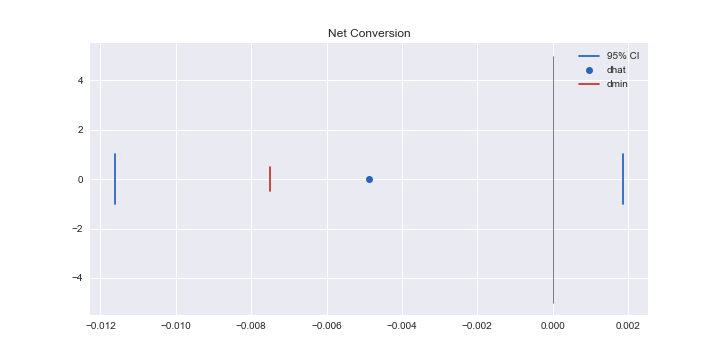
\includegraphics[width=\textwidth]{net_conv}

\subsubsection{Sign Test}

In order to perform the sign test, the number of days with a positive change, i.e. the gross and net conversion of the experiment group is greater than those of the control group, are counted. The results are
\begin{labeling}{Gross Conversion}
\item[Gross Conversion] Number of successes: 4, total number days: 23
\item[Net Conversion] Number of successes: 10, total number days: 23
\end{labeling}

Using \url{http://graphpad.com/quickcalcs/binomial1.cfm}, this gives the following two-tail P values:
\begin{eqnarray}
	p_{GC} &=& .0026 < \alpha = .05\\
      p_{NC} &=& .6776 > \alpha = .05
\end{eqnarray}
This indicates that gross conversion is statistically significant whereas net conversion is not.

\subsubsection{Summary}

Bonferroni correction was not used, as two metrics (gross and net conversion) are considered and the prerequisite for launching the change is a reduced gross conversion \textit{and} a net conversion that does not decrease. This means an increased risk for a Type II error (false negatives); Bonferroni correction on the other hand is intended to reduce the risk of Type I error (false positives). Hence, it is not applicable here.

The effect size tests yields that gross conversion is statistically and practically significant. Net conversion is neither. The statistical significance of gross conversion is confirmed by the sign test. It also shows that net conversion is not statistically significant.

\subsection{Recommendation}

The experiment shows that the number of students to enroll in the 14-day trial are effectively reduced, which was one of the goals. However, at the same time the number of students to continue past the free trial and make at least one payment should not be reduced. This could not be shown in the experiment as the practical significance boundary for net conversion ($d_{min} = .0075$) falls within the confidence interval. So, there is a risk that the proposed change also negatively affects the number of students to make a payment. Therefore, the recommendation is not to launch the change.

\section{Follow-Up Experiment}

The initial experiment proved successful in terms of reducing the number of students to enrol in the free trial. However, it seems that it also reduces the number of students to continue past the 14-day trial. It is possible that there a students that initially indicate that they would spend more than 5 hours per week but for whatever reason do not invest the required amount of time. \medskip

The follow-up experiment could consist in a check after the first week; if a student spends less than 5 hours, another screener is displayed to ask whether the student would like to schedule a one-to-one meeting with a coach. The idea is that this motivates the student to invest more time in the second week and subsequently continues past the free trial.\medskip

As this concerns only students that have already enrolled in the free trial, the \textbf{Unit of Diversion} would be User ID. User ID would also be an \textbf{Invariant Metric}, as the numbers of users to enrol in the free trial should not be impacted by the experiment. The metric for the follow-up experiment would be \textbf{Retention}, as the goal would be to see an increased number of students to make a payment.

\end{document}